\chapter{Experimental setup}

A common strategy to study \B meson decays is by dedicated colliders, known as $B$ factories.
$B$ factory experiments operate by producing large quantities of \BB pairs, usually by producing \FourS mesons that primarily decay to two \B meson pairs (\BB) \cite{Workman:2022ynf}.
Historically, three $B$ factory experiments operated:
\begin{itemize}
    \item CLEO with the CESR accelerator at Cornell University, USA;
    \item BaBar with the PEP-II accelerator at SLAC, USA;
    \item Belle with KEKB accelerator at KEK, Japan.
\end{itemize}
Although not a $B$ factory, another experiment, known as LHCb, with the LHC accelerator at CERN, collects data from $B$ mesons that are produced in proton-proton collisions.
It has been running since 2008 and is still in operation.

The three aforementioned $B$ factory experiments have since completed their operation.
However, an upgraded version of Belle, known as Belle~II, began collecting data in 2018.
Belle~II is a detector at the KEK laboratory in Tsukuba, Japan.
Its main purpose it the collection of electron-positron (\epem) collision data 
at the center of mass energies ($\sqrt{s}$) at or near the \FourS meson mass.
The colliding beams are provided by the SuperKEKB \epem collider.
This chapter provides an overview of Belle II and introduces the mains concepts of the SuperKEKB accelerator.

\todo[inline]{add quotes, also maybe mention that cleo wasnt origiinally a b factory.}

\section{The SuperKEKB accelerator}

The SuperKEKB accelerator, discussed in detail in Ref.\cite{Akai:2018mbz}, is a double-ring electron-positron collider.
It is an upgraded version of the KEKB collider \cite{Oide:2009zz} that operator with the Belle experiment, a predecessor to Belle~II.
The SuperKEKB accelerator complex is schematically shown in \Cref{fig:superkekb}.
A photo-cathode radio-frequency gun produces the electrons, which are then subsequently accelerated to 7~\gev by a linear accelerator into the electron ring.
On the other hand, protons are created by directing an electron beam to a tungsten target.
%, producing bremmstrahlung photons which create electron and positron pairs.
The positrons are singled out using the magnetic field and accelerated to 1.1~\gev, injected them into the damping ring and, finally,
accelerated by the linear accelerator to 4~\gev before the injection to the positron ring.
The subsequent collision occurs inside the Belle~II detector, where the two electron and positron rings meet.
\begin{figure}[htbp!]
    \centering
    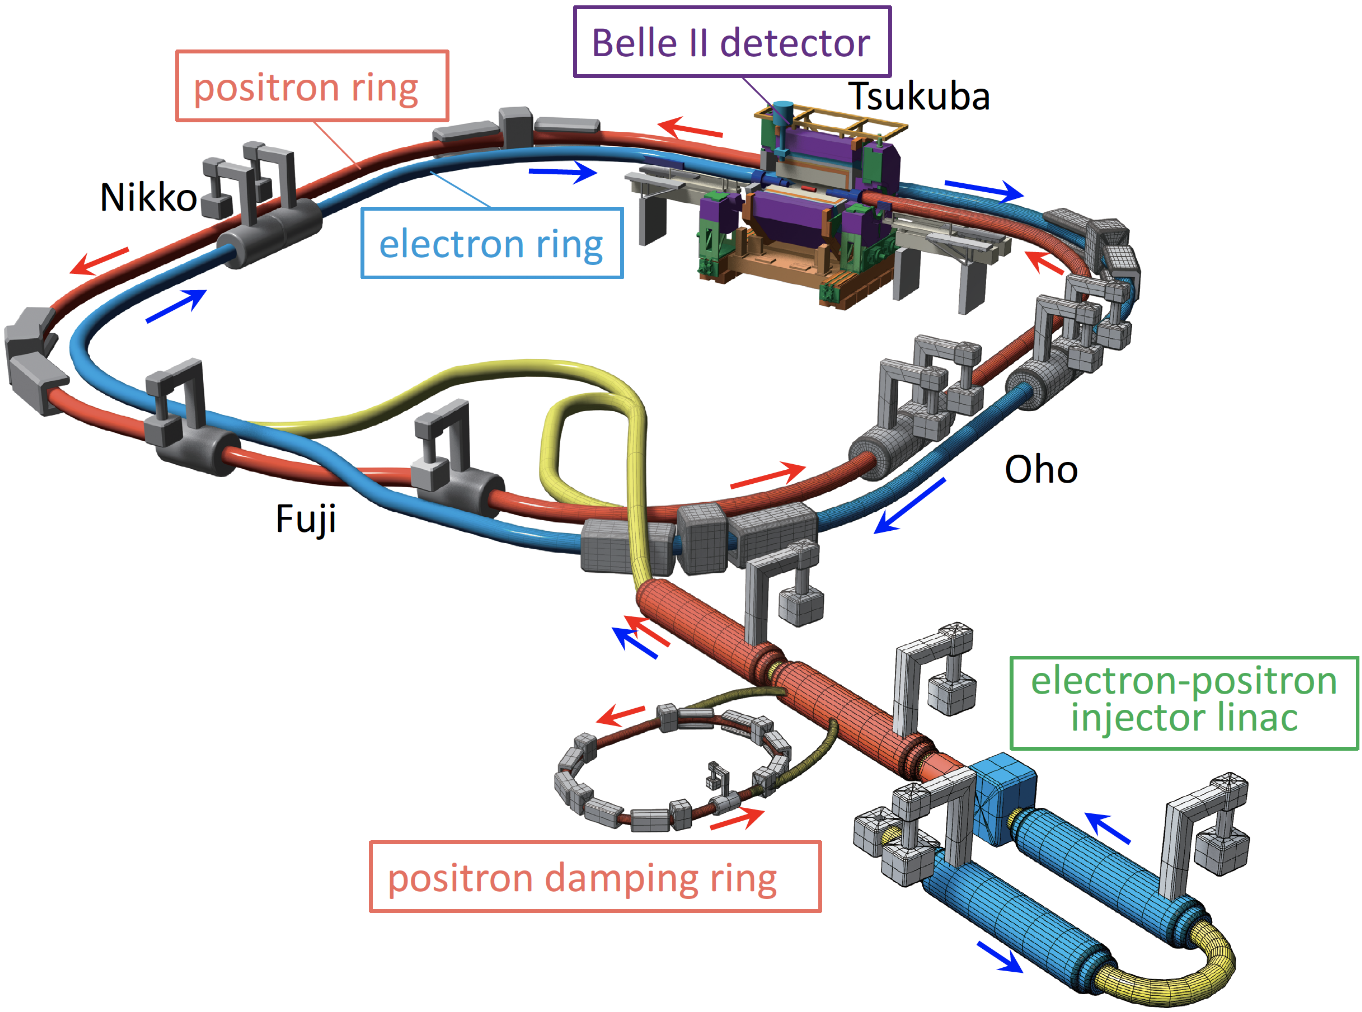
\includegraphics[width=0.6\textwidth]{figures/experimental_setup/super_kekb.png}
    \caption{\label{fig:superkekb}
        The schematic visualisation of the SuperKEKB accelerator complex.
        The main components that contribute to the acceleration of electrons and positrons are shown.
        The four straight sections are named after Japanese cities.
        Credit to \cite{Akai:2018mbz}.
    }
\end{figure}

The beam-energy asymmetry (7~\gev for \en and 4~\gev for \ep) is an important design characteristic of SuperKEKB, 
which allows to separate $B$ meson vertices, necessary for measurements such as time-dependent CP violation \cite{BaBar:2014omp}.
On the other hand, the exact collision energy is chosen in order to operate at the $m(\FourS)\approx10.58~\gev$ energy, 
hence fulfilling the requirements of the $B$ factory experiment.

Interestingly \epem collision at $10.58~\gev$ produces more than just \FourS.
In truth, amny other decay products including $\epem\ra\ell^+\ell^-$ or $\epem\ra\qqbar$ proceses may occur and the production 
cross-section  of all these processes depends on $\sqrt{s}$.
This is shown in XXXX.

